\chapter{Work Plan}
\label{c3}

This chapter presents the work plan for my thesis.
The goal is to develop a language model that generates answers to consumer health questions with adjustable complexity levels.
The model should be able to produce simple and concise answers for non-experts, as well as detailed and technical responses for healthcare professionals.

This plan is structured around three core research questions (RQ), with detailed tasks and a timeline spanning from January to June 2025. 
The timeline is provisional and may change based on progress or unforeseen challenges.

\section{Research Questions}
To guide the development of the controllable health QA model, we define the following research questions:

\subsection*{RQ1: What combination of metrics best captures the complexity of medical text?}

To generate answers at different complexity levels, we first need to figure out how to measure text complexity in the medical domain. 
There are existing readability formulas like \gls{fkgl}, but they do not capture all the aspects that make medical text hard to understand, like specialized vocabulary and complex sentence structures. 
The goal is to find the combination of metrics that does the best job distinguishing simple and complex medical writing in a way that aligns with human judgment.


\subsubsection*{Task 1.1: Literature Review:}

\begin{itemize}
    \item Conduct a thorough review of existing literature on readability metrics and complexity measures tailored for health-related text.
    \item Identify the most promising metrics and measures to be used in the project.
\end{itemize}

\subsubsection*{Task 1.2: Dataset Preparation}

\begin{itemize}
    \item Search for and acquire a dataset containing paired examples of complex and simplified health articles or documents.
    \item Preprocess the dataset, ensuring it is clean, well-structured, and ready for analysis.
\end{itemize}

\subsubsection*{Task 1.3: Metric Selection and Evaluation}

\begin{itemize}
    \item Implement the selected readability metrics and complexity measures identified in Task 1.1.
    \item Calculate the complexity scores for each text pair in the preprocessed dataset.
    \item Select the combination of metrics that best distinguishes between complex and simple texts based on the results of the Kullback-Leibler (KL) divergence, clustering (e.g., K-means), and classification (e.g., logistic regression) experiments.
\end{itemize}

\paragraph{Milestone 1:} Development of a robust method for quantifying the complexity of health-related text.

\subsection*{RQ2: How do we create good training dataset for complexity controlled text generation?}

To train a model to output answers at different complexity levels, we first need a dataset that exhibits this type of variance.
Since there aren't any datasets like this, we'll need to create our own by collecting medical text from various sources and annotating it with the set of metrics identified in RQ1.

\subsubsection*{Task 2.1: Data Collection}

\begin{itemize}
    \item Identify a suitable dataset of expert-level health question-answer pairs.
    \item Preprocess the dataset, ensuring it is clean, well-structured, and ready for use.
\end{itemize}

\subsubsection*{Task 2.2: Answer generation using pre-trained models}

\begin{itemize}
    \item Select and set up a pre-trained language model, such as BioBERT or SciBERT, for answer generation.
    \item Feed the question and reference answer into the chosen pre-trained model and prompt it to generate several alternative answers, ranging from very simple to highly complex.
\end{itemize}

\subsubsection*{Task 2.3: Dataset Annotation}

\begin{itemize}
    \item Apply the complexity quantification method developed in RQ1 to the generated answers.
    \item Create a complexity-stratified dataset by labeling each generated answer with its corresponding complexity level.
\end{itemize}

\subsubsection*{Task 2.4: Answer Validation}

\begin{itemize}
    \item Validate the generated answers to ensure they are factually accurate and relevant to the original questions.
    \item Remove any low-quality or irrelevant answers from the dataset.
\end{itemize}

\paragraph{Milestone 2:} Curation of a high-quality dataset of health question-answer pairs with annotated complexity levels.


\subsection*{RQ3: How can we design a language model that reliably generates health answers with adjustable complexity levels?}

With the labeled dataset from RQ2, we can train a language model to generate answers at different complexity levels based on what the user asks for. 
There are a few different approaches we could try, like fine-tuning the model on the labeled data, manipulating the model's latent representations, or using reinforcement learning to reward outputs that match the target complexity. 
The challenge is to find the method that gives the best control over complexity while still producing accurate and relevant answers.

\subsubsection*{Task 3.1: Fine-tuning Baseline Model}

\begin{itemize}
    \item Fine-tune a pre-trained language model, such as BioBERT or SciBERT, on the complexity-stratified dataset created in RQ2.
    \item Establish a baseline performance for complexity-controlled answer generation.
\end{itemize}

\subsubsection*{Task 3.2: Exploring Advanced Techniques}

\begin{itemize}
    \item Investigate and implement advanced techniques for controllable text generation, such as latent space manipulation, reinforcement learning, or adversarial training.
    \item Experiment with different approaches and hyperparameters to optimize the model's performance.
    \item Combine multiple controllable generation techniques to see if they yield cumulative improvements.
\end{itemize}

\subsubsection*{Task 3.3: Evaluation and Validation}

\begin{itemize}
    \item Evaluate the performance of the developed models using a combination of automatic metrics and human evaluation.
    \item Assess the models' ability to control complexity, generate factually accurate and relevant answers, and produce fluent and coherent text.
\end{itemize}

\subsubsection*{Task 3.4: (Optional) Integrate external knowledge bases}

\begin{itemize}
    \item Investigate the feasibility of integrating external knowledge bases, such as PubMed or Wikipedia, to improve the model's understanding of medical concepts and terminology.
    \item Implement a knowledge retrieval mechanism to provide additional context and information for answer generation.
    \item Evaluate the impact of external knowledge integration on the model's performance and answer quality.
\end{itemize}

\paragraph{Milestone 3:} Development of a controllable language model for generating health answers with adjustable complexity levels.

\section{Timeline}

The following Gantt chart provides a visual representation of the proposed work plan, outlining the tasks and milestones described above, along with other related activities such as writing the final thesis document.

\begin{figure}[!htbp]
    \centering
    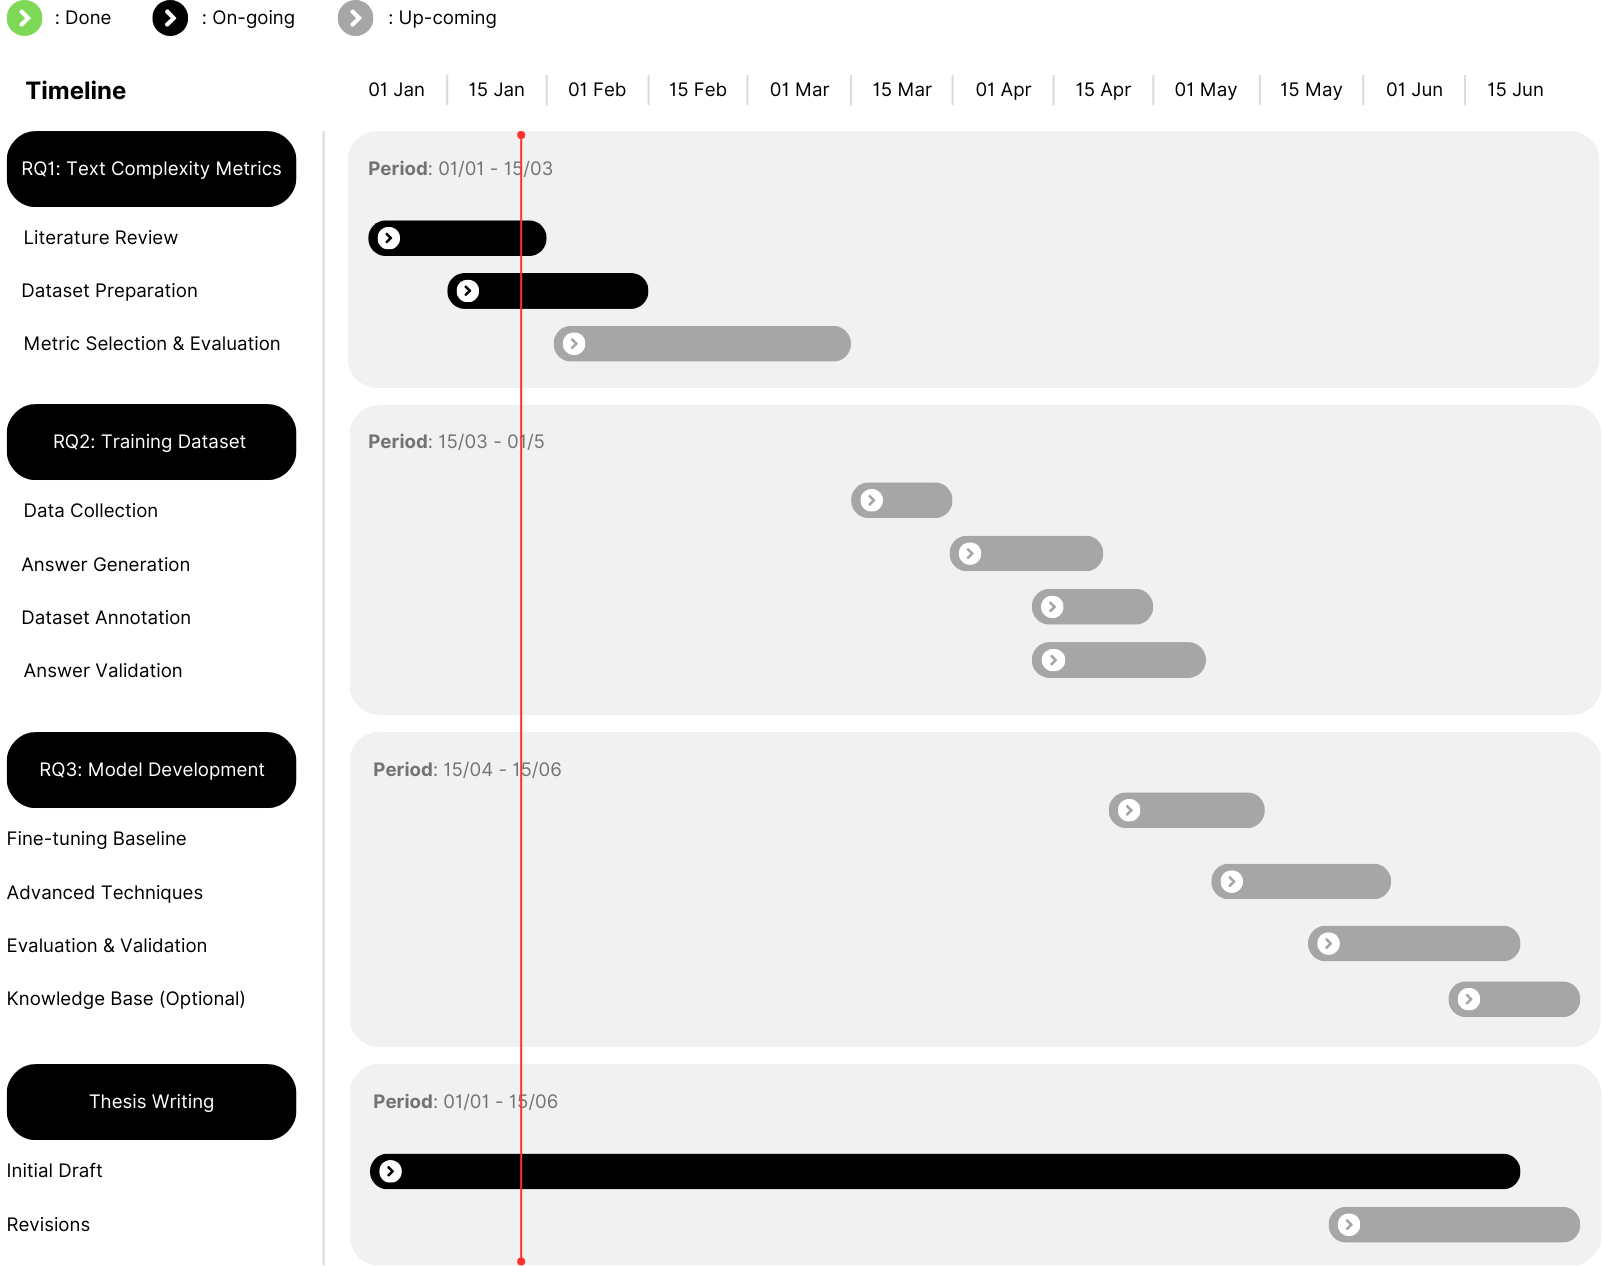
\includegraphics[width=\textwidth]{img/timeline.png}
    \caption{Proposed timeline for the thesis project.}
    \label{fig:gantt}
\end{figure}

The models will be trained using the Pleiades High Performance Computing (HPC) cluster operated by IEETA. As this is a new setup and I have limited experience with training large language models, the exact timeline may need to be adjusted as the project progresses.